\documentclass[a4paper]{article}
\usepackage{a4wide,amssymb,epsfig,latexsym,multicol,array,hhline,fancyhdr}
%\usepackage{vntex}
\usepackage{amsmath}
\usepackage{lastpage}
\usepackage[lined,boxed,commentsnumbered]{algorithm2e}
\usepackage{enumerate}
\usepackage{color}
\usepackage{graphicx}							% Standard graphics package
\usepackage{array}
\usepackage{tabularx, caption}
\usepackage{multirow}
\usepackage{multicol}
\usepackage{rotating}
\usepackage{graphics}
\usepackage{graphicx}
\usepackage{geometry}
\usepackage{setspace}
\usepackage{epsfig}
\usepackage{tikz}
\usepackage{amsmath}
\usepackage{listings}
\usepackage{xcolor}
\usetikzlibrary{arrows,snakes,backgrounds}
\usepackage{hyperref}
\hypersetup{urlcolor=blue,linkcolor=black,citecolor=black,colorlinks=true} 
%\usepackage{pstcol} 								% PSTricks with the standard color package
\usepackage{float}
\usepackage[none]{hyphenat}

\newtheorem{theorem}{{\bf Theorem}}
\newtheorem{property}{{\bf Property}}
\newtheorem{proposition}{{\bf Proposition}}
\newtheorem{corollary}[proposition]{{\bf Corollary}}
\newtheorem{lemma}[proposition]{{\bf Lemma}}

\AtBeginDocument{\renewcommand*\contentsname{Contents}}
\AtBeginDocument{\renewcommand*\refname{References}}
%\usepackage{fancyhdr}
\setlength{\headheight}{40pt}
\pagestyle{fancy}
\fancyhead{} % clear all header fields
\fancyhead[L]{
 \begin{tabular}{rl}
    \begin{picture}(25,15)(0,0)
    \put(0,-8){
\includegraphics[width=8mm, height=8mm]{hcmut.png}}
    %\put(0,-8){\epsfig{width=10mm,figure=hcmut.eps}}
   \end{picture}&
	%
\includegraphics[width=8mm, height=8mm]{hcmut.png} & %
	\begin{tabular}{l}
		\textbf{\bf \ttfamily University of Technology, Ho Chi Minh City}\\
		\textbf{\bf \ttfamily Faculty of Computer Science and Engineering}
	\end{tabular} 	
 \end{tabular}
}
\fancyhead[R]{
	\begin{tabular}{l}
		\tiny \bf \\
		\tiny \bf 
	\end{tabular}  }
\fancyfoot{} % clear all footer fields
\fancyfoot[L]{\scriptsize \ttfamily Machine Learning - Semester 1 (2023 - 2024)}
\fancyfoot[R]{\scriptsize \ttfamily Page {\thepage}/\pageref{LastPage}}
\renewcommand{\headrulewidth}{0.3pt}
\renewcommand{\footrulewidth}{0.3pt}


%%%
\setcounter{secnumdepth}{4}
\setcounter{tocdepth}{3}
\makeatletter
\newcounter {subsubsubsection}[subsubsection]
\renewcommand\thesubsubsubsection{\thesubsubsection .\@alph\c@subsubsubsection}
\newcommand\subsubsubsection{\@startsection{subsubsubsection}{4}{\z@}%
                                     {-3.25ex\@plus -1ex \@minus -.2ex}%
                                     {1.5ex \@plus .2ex}%
                                     {\normalfont\normalsize\bfseries}}
\newcommand*\l@subsubsubsection{\@dottedtocline{3}{10.0em}{4.1em}}
\newcommand*{\subsubsubsectionmark}[1]{}
\makeatother

% Define colors for code listing
\definecolor{codegreen}{rgb}{0,0.6,0}
\definecolor{codegray}{rgb}{0.5,0.5,0.5}
\definecolor{codepurple}{rgb}{0.58,0,0.82}
\definecolor{backcolour}{rgb}{0.95,0.95,0.92}

% Code listing style
\lstdefinestyle{mystyle}{
	backgroundcolor=\color{backcolour},   
	commentstyle=\color{codegreen},
	keywordstyle=\color{magenta},
	numberstyle=\tiny\color{codegray},
	stringstyle=\color{codepurple},
	basicstyle=\ttfamily\footnotesize,
	breakatwhitespace=false,         
	breaklines=true,                 
	captionpos=b,                    
	keepspaces=true,                 
	numbers=left,                    
	numbersep=5pt,                  
	showspaces=false,                
	showstringspaces=false,
	showtabs=false,                  
	tabsize=2
}

\lstset{style=mystyle}
\begin{document}

\begin{titlepage}
\begin{center}
VIETNAM NATIONAL UNIVERSITY, HO CHI MINH CITY \\
UNIVERSITY OF TECHNOLOGY \\
FACULTY OF COMPUTER SCIENCE AND ENGINEERING
\end{center}

\vspace{1cm}

\begin{figure}[h!]
\begin{center}

\includegraphics[width=3cm]{hcmut.png}
\end{center}
\end{figure}

\vspace{1cm}


\begin{center}
\begin{tabular}{c}
\multicolumn{1}{l}{\textbf{{\Large Machine Learning - CO3117}}}\\
~~\\
\hline
\\
\multicolumn{1}{l}{\textbf{{\Large Assignment}}}\\\\
\\
\textbf{{\Huge Iris Flower Classification}}\\
\multicolumn{1}{l}
\textbf{{\Huge using several Machine Learning models}}\\
\\\\
\hline
\end{tabular}
\end{center}

\vspace{3cm}

\begin{table}[h]
\begin{tabular}{rrl}
\hspace{3 cm} & \textbf{{\ Instructor}}: & Nguyen Duc Dung \\
\hspace{3 cm} & \textbf{{\ Class}}: & CC01  \\
\hspace{3 cm} & \textbf{{\ Student}}: 
& Tran Anh Kiet - 2152147 \\ 
\\

& &   \\
& &   \\
\end{tabular}
\end{table}

\begin{center}
{\footnotesize HO CHI MINH CITY, DECEMBER 2023}
\end{center}
\end{titlepage}


%\thispagestyle{empty}

\newpage
	\tableofcontents
\newpage

\section{Introduction}
Irises influenced the design of the French fleur-de-lis, are commonly used in the Japanese art of flower arrangement known as Ikebana, and underlie the floral scents of the “essence of violet” perfume. They’re also the subject of this well-known machine learning project, in which you must create an ML model capable of sorting irises based on five factors into one of three classes, Iris Setosa, Iris Versicolour, and Iris Virginica.

To get started, the data set below includes 50 instances of each of the three iris classes for a total of 150 instances. While one of the classes is linearly separable, the other two are not. Our goal is to create a model capable of classifying each iris instance into the appropriate class based on four attributes: sepal length, sepal width, petal length, and petal width. 
\begin{figure}[h]
	\centering
	\begin{minipage}{0.32\textwidth}
		\centering
		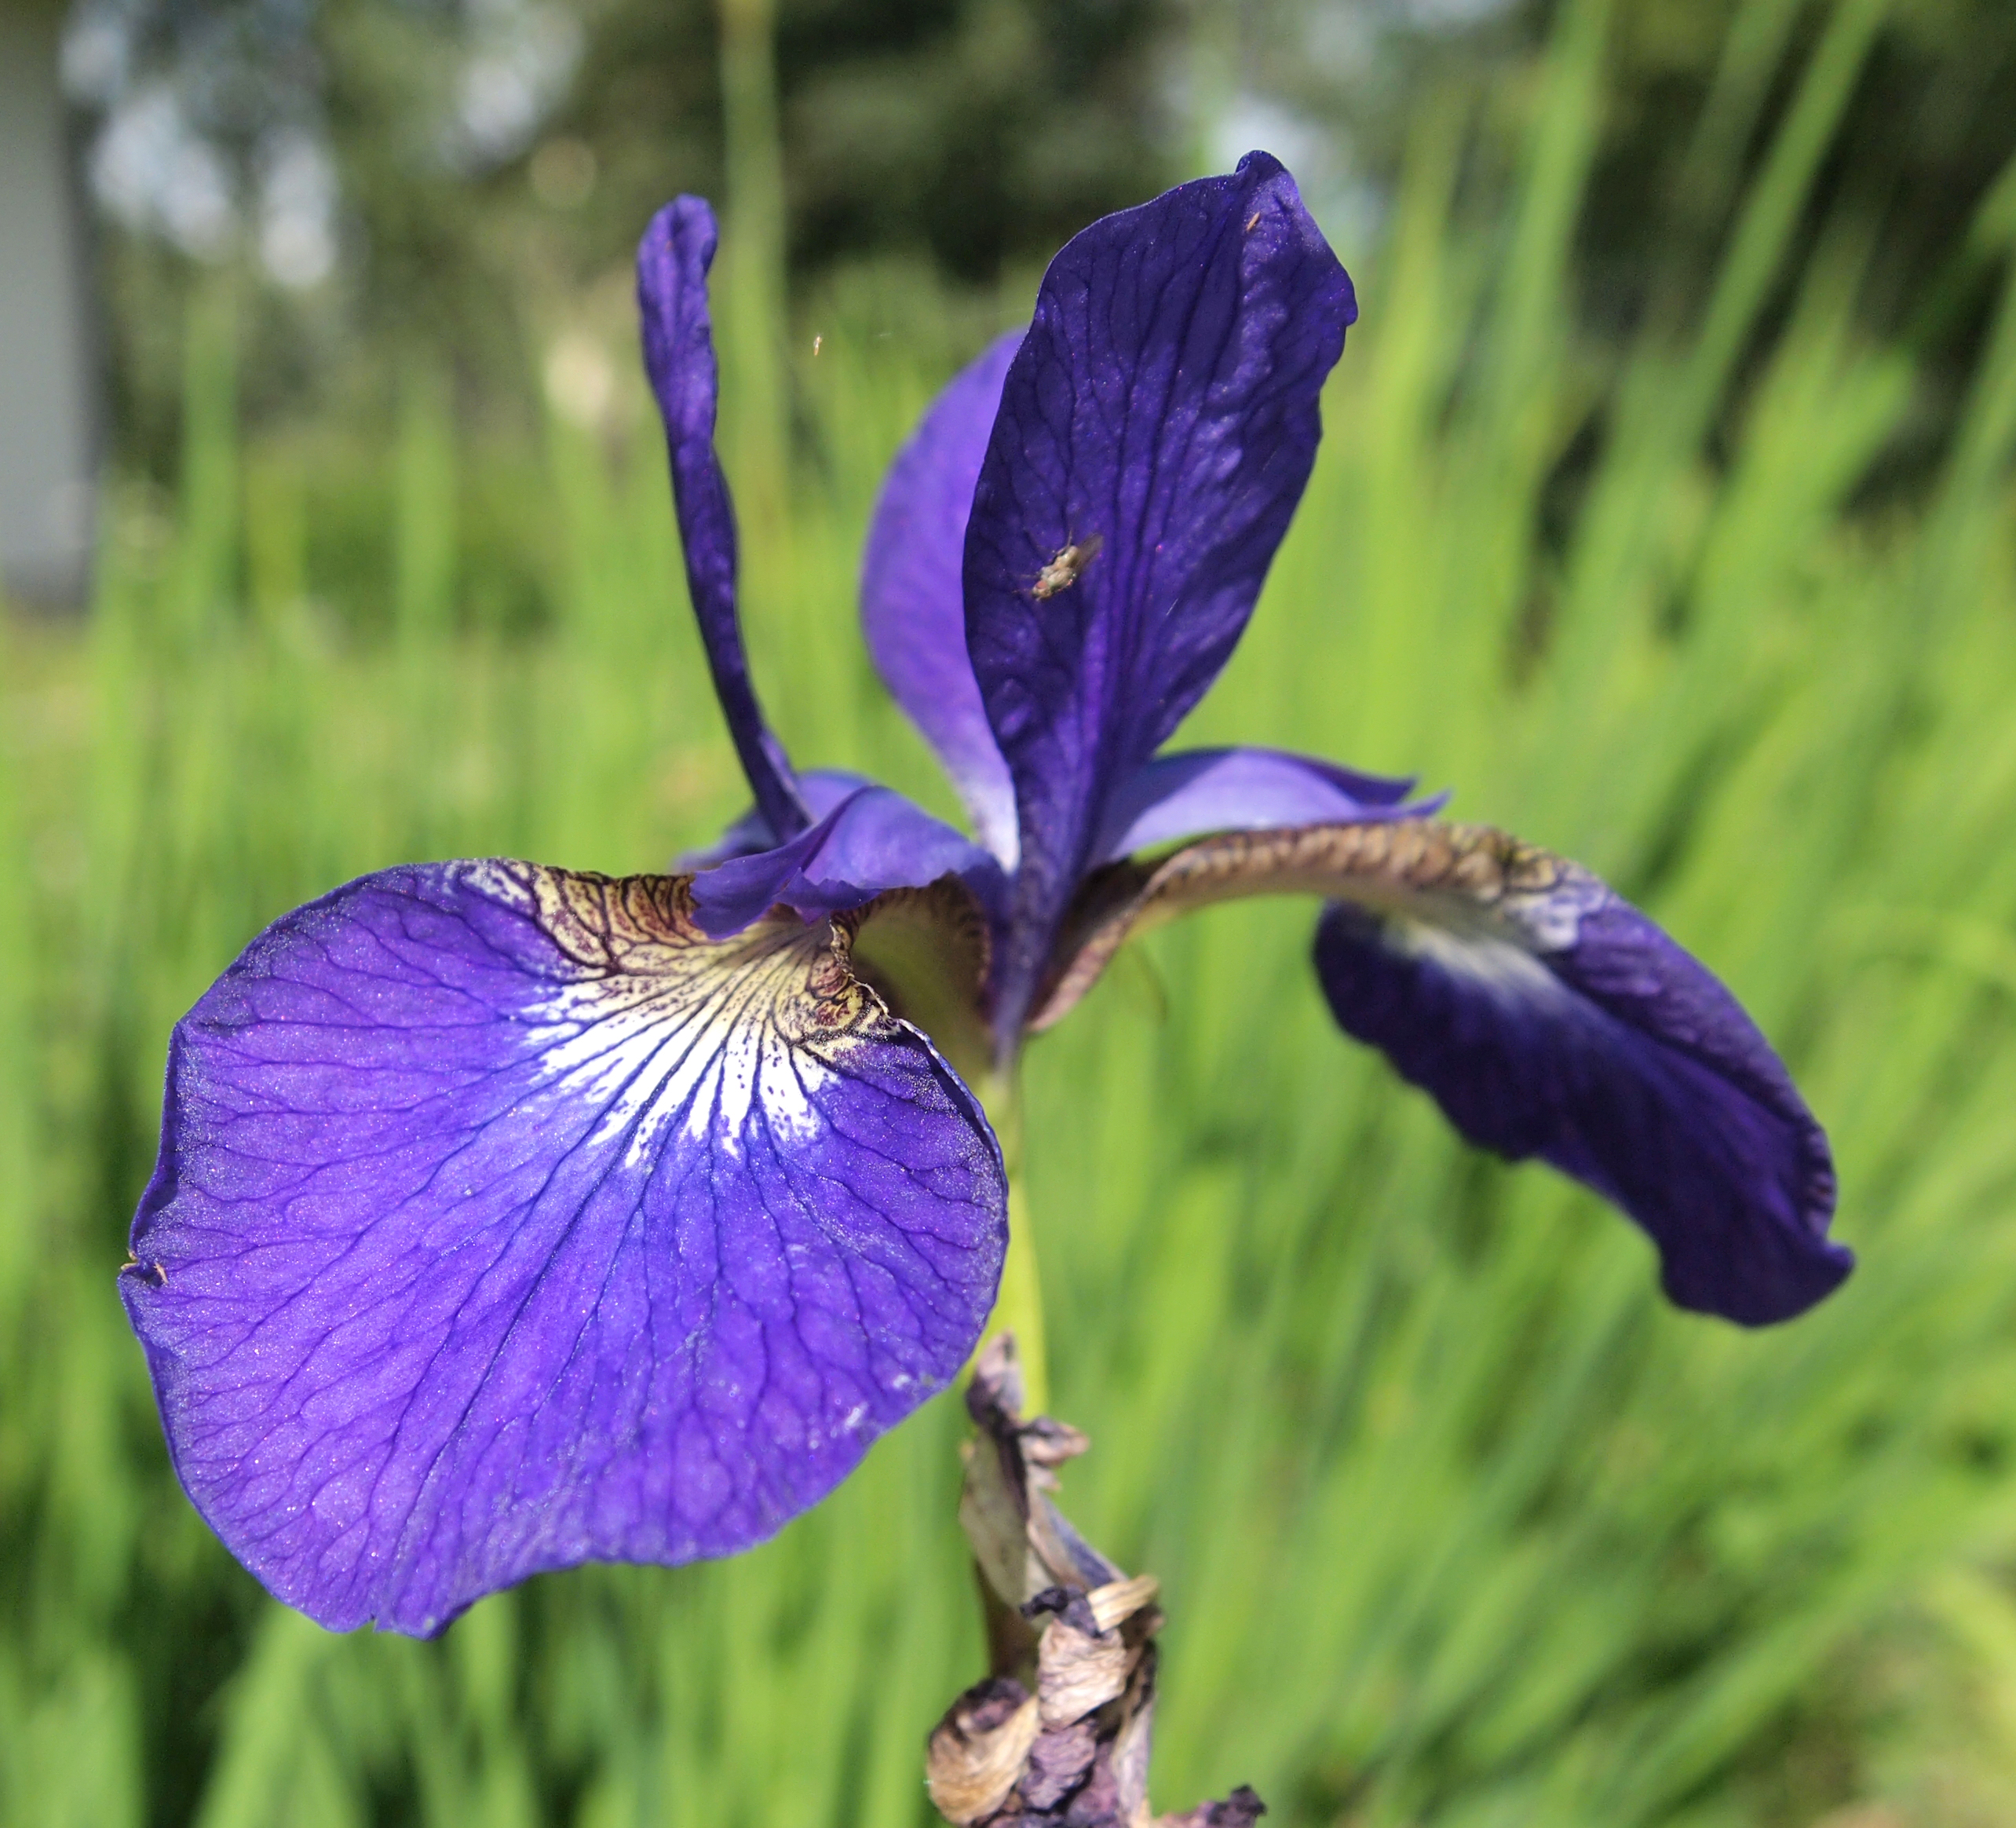
\includegraphics[height=4cm]{picture/flower/Iris Setosa} % Adjust height as needed
		\caption{Iris Setosa}
		\label{fig:setosa}
	\end{minipage}\hfill
	\begin{minipage}{0.32\textwidth}
		\centering
		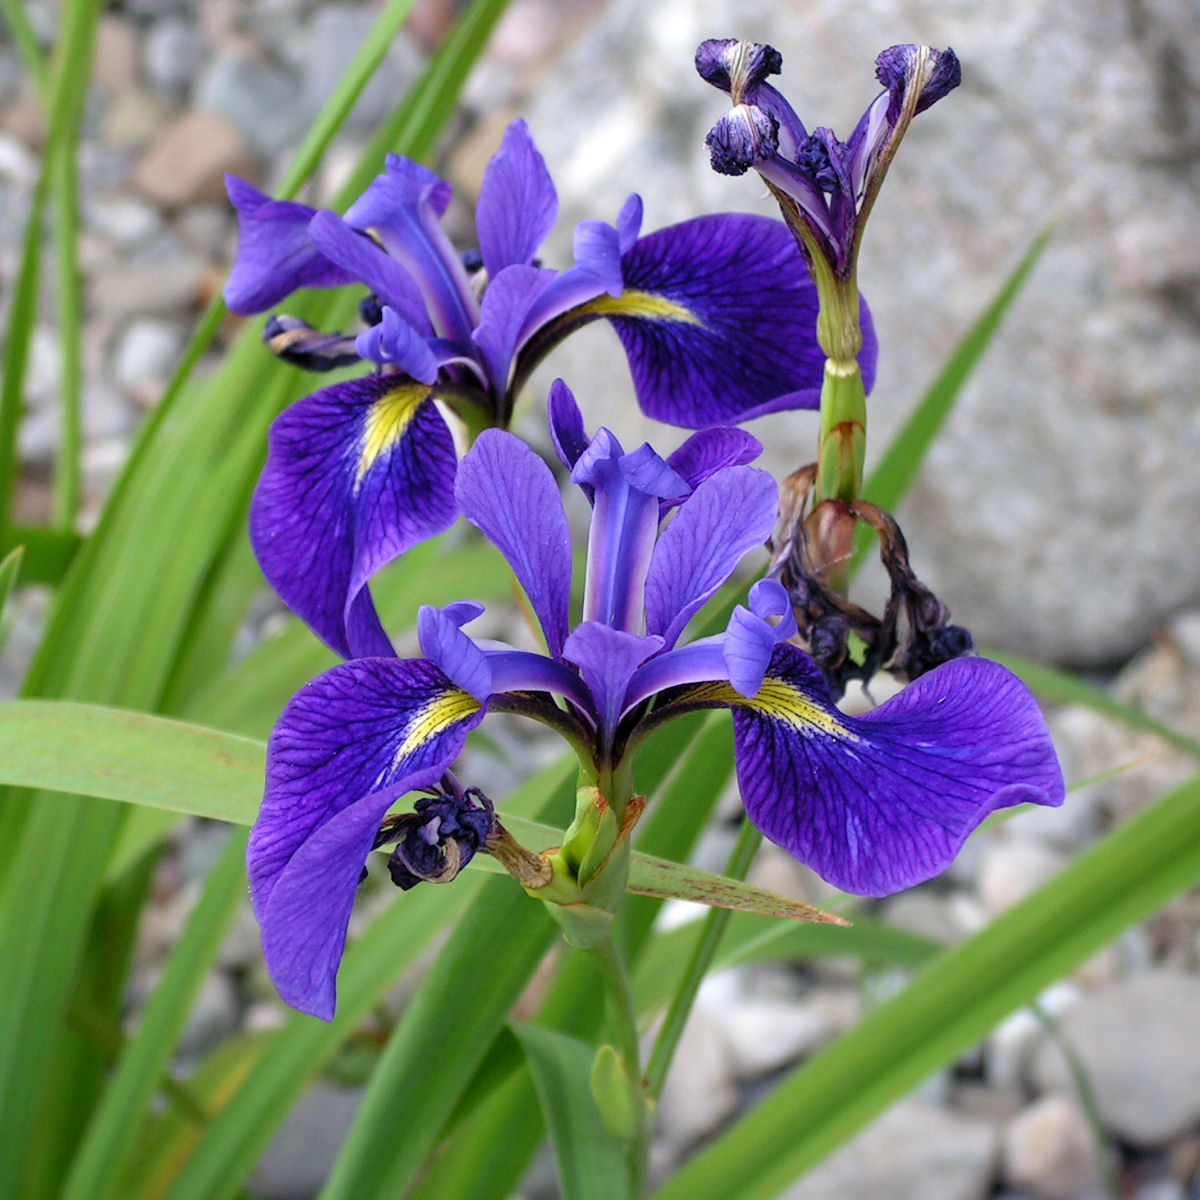
\includegraphics[height=4cm]{picture/flower/Iris Versicolour} % Adjust height as needed
		\caption{Iris Versicolour}
		\label{fig:versicolour}
	\end{minipage}\hfill
	\begin{minipage}{0.32\textwidth}
		\centering
		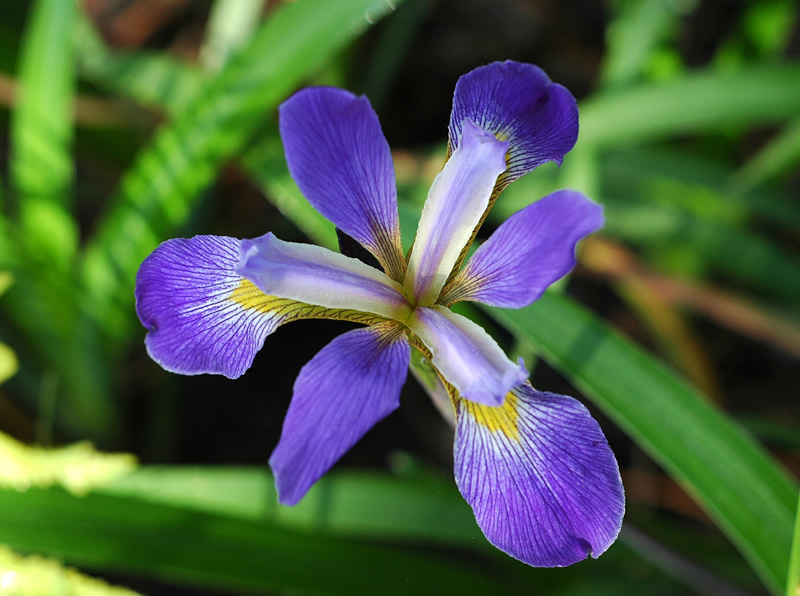
\includegraphics[height=4cm]{picture/flower/Iris Virginica} % Adjust height as needed
		\caption{Iris Virginica}
		\label{fig:virginica}
	\end{minipage}
\end{figure}

\section{Literature Review}
Discuss previous work and findings related to the Iris classification problem.
For classifying, i use 3 polular model in machine learning
\subsection{Machine Learning Models Used in This Project}
\begin{enumerate}
	\item \textbf{K-nearest Neighbors}
	The K-Nearest Neighbors (K-NN) algorithm is one of the simplest machine learning algorithms, based on the supervised learning technique. It assumes similarity between the new case/data and available cases, categorizing the new case into the most similar available category. K-NN stores all available data and classifies new data points based on similarity, making it a convenient method for classifying new data into suitable categories.
	
	K-NN can be used for both regression and classification, though it is primarily used for classification problems. It is a non-parametric algorithm, meaning it does not make any assumptions about the underlying data distribution. Also known as a lazy learner algorithm, K-NN does not immediately learn from the training set but rather stores the dataset and performs actions upon classification.
	
	For example, consider two categories, Category A and Category B. If we have a new data point x1, K-NN helps determine whether this data point belongs to Category A or B. The process can be visualized in the diagram below:
	\begin{figure}[h]
		\centering
		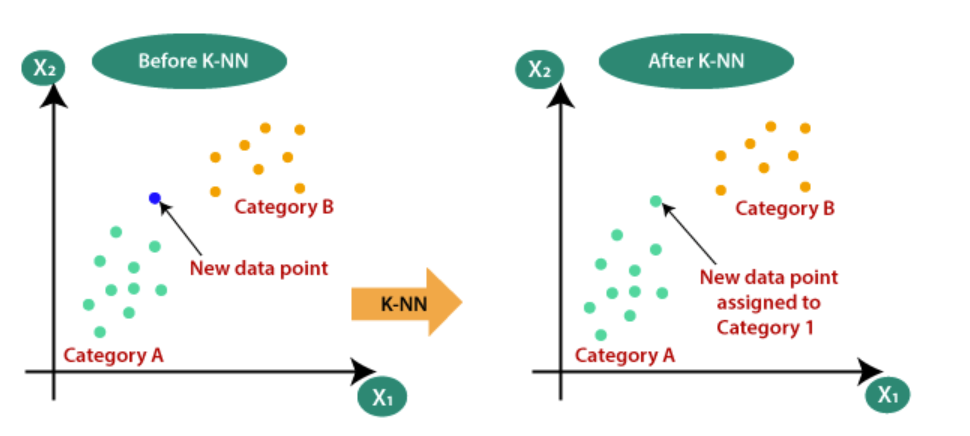
\includegraphics[width=1\textwidth]{picture/KNN1}
		\caption{Illustration of K-NN Classification}
		\label{fig:knn1}
	\end{figure}
	
	\textbf{How Does K-NN Work?}
	The K-NN algorithm operates as follows:
	
	\begin{enumerate}
		\item Select the number K of neighbors.
		\item Calculate the Euclidean distance of K neighbors.
		\item Take the K nearest neighbors as per the Euclidean distance.
		\item Count the number of data points in each category among these K neighbors.
		\item Assign the new data points to the category with the maximum number of neighbors.
		\item The model is ready.
	\end{enumerate}
	Suppose we have a new data point that needs categorization. First, we choose the number of neighbors (k=5). Next, we calculate the Euclidean distance between the data points, as shown below:
	\begin{figure}[h]
		\centering
		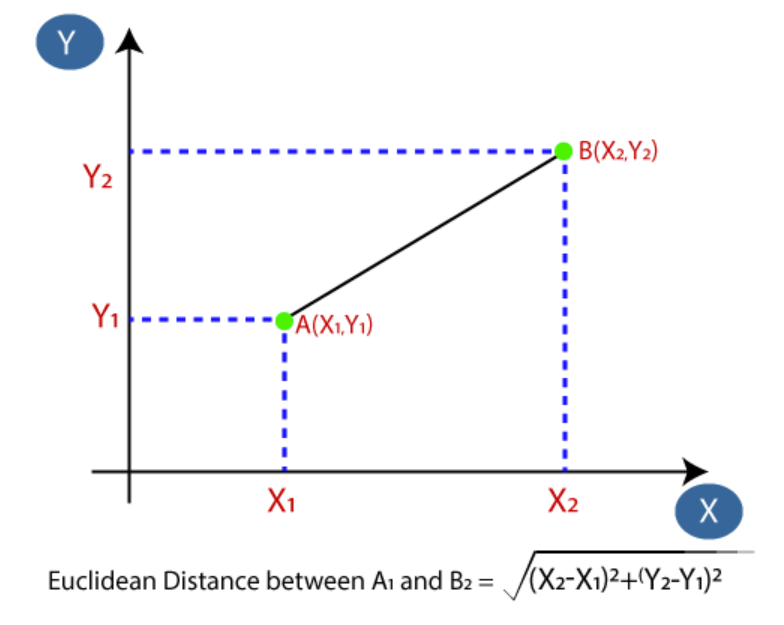
\includegraphics[width=0.5\textwidth]{picture/KNN2}
		\caption{Euclidean Distance Calculation in K-NN}
		\label{fig:knn2}
	\end{figure}
	
	After calculating the Euclidean distance, we identify the nearest neighbors. For instance, if there are three nearest neighbors in Category A and two in Category B, as illustrated in the image below, the new data point would most likely belong to Category A.
	\begin{figure}[h]
		\centering
		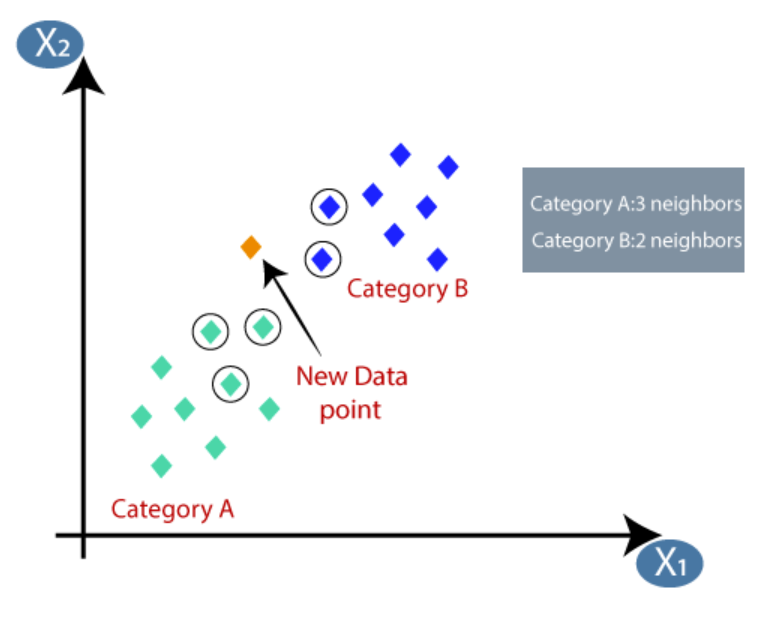
\includegraphics[width=0.5\textwidth]{picture/KNN3}
		\caption{Identifying Nearest Neighbors in K-NN}
		\label{fig:knn3}
	\end{figure}
	
	\item \textbf{Random Forest}
	\item \textbf{Logistic Regression}
\end{enumerate}

\subsection{Confusion Matrix}
A confusion matrix is a table typically used to describe the performance of a classification model on a set of test data for which the true values are known. It visualizes the model's accuracy by comparing the actual target values with the predictions made by the machine learning model.

Consider the following example of a confusion matrix:
\begin{figure}[h]
	\centering
	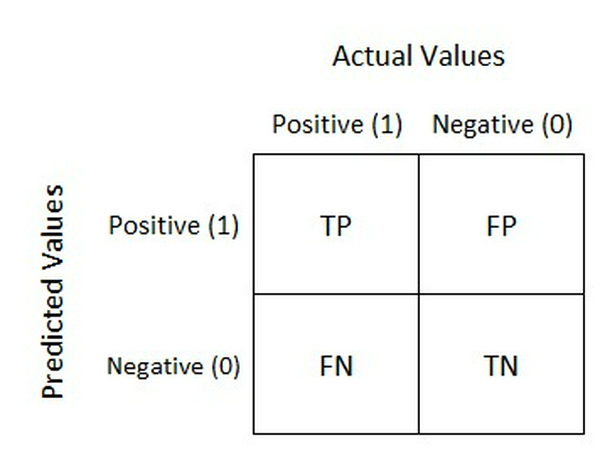
\includegraphics[width=0.5\textwidth]{picture/confusion}
	\caption{Confusion Matrix Example}
	\label{fig:confusion_matrix}
\end{figure}

The key components of a confusion matrix are:
\begin{itemize}
	\item \textbf{True Positive (TP)}: Instances where the model correctly predicts the positive class.
	\item \textbf{True Negative (TN)}: Instances where the model correctly predicts the negative class.
	\item \textbf{False Positive (FP)}: Instances where the model incorrectly predicts the positive class, also known as a Type I error.
	\item \textbf{False Negative (FN)}: Instances where the model incorrectly predicts the negative class, also known as a Type II error.
\end{itemize}

In the case of a multi-class classification problem, such as the Iris dataset, the confusion matrix will have dimensions of \( n\_classes \times n\_classes \). Each entry (i, j) in the matrix corresponds to the number of instances where class i was predicted as class j.

\subsection{Classification Report}
The classification report presents several key metrics for each class, which are essential for evaluating the performance of a classification model:

\begin{itemize}
	\item \textbf{Precision}: This metric is the ratio of correctly predicted positive observations to the total predicted positives. It addresses the question, "Of all instances labeled as positive by the model, how many are actually positive?" Precision is calculated as TP / (TP + FP), where TP is the number of true positives and FP is the number of false positives.
	
	\item \textbf{Recall} (also known as Sensitivity or True Positive Rate): Recall is the ratio of correctly predicted positive observations to all observations in the actual class. It answers the question, "Of all the instances that are actually positive, how many were correctly labeled by the model?" It is calculated as TP / (TP + FN), where FN is the number of false negatives.
	
	\item \textbf{F1-Score}: This score is the weighted harmonic mean of precision and recall. It considers both false positives and false negatives, making it a robust measure that shows the balance between precision and recall. The F1-Score is calculated as 2 * (Precision * Recall) / (Precision + Recall).
	
	\item \textbf{Support}: This indicates the number of actual occurrences of each class in the specified dataset. For instance, if Iris-setosa has a support of 11, it means there are 11 instances of Iris-setosa in the test set that the model has attempted to predict.
	
	\item \textbf{Accuracy}: Accuracy represents the ratio of correctly predicted observations to the total observations. It is expressed as (TP + TN) / Total, where TN is the number of true negatives.
	
	\item \textbf{Macro Average}: This is the average of precision, recall, and F1-score calculated between classes, without considering class imbalance. It gives equal weight to each class.
	
	\item \textbf{Weighted Average}: In contrast to the macro average, the weighted average of precision, recall, and F1-score is calculated between classes while taking into account the number of instances in each class. This approach weights each class proportionally to its presence in the dataset.
\end{itemize}

\section{Methodology}
\subsection{Data Collection}
The dataset was obtained from the UCI Machine Learning Repository. For more information, visit the \href{https://archive.ics.uci.edu/ml/datasets/iris}{UCI Iris Dataset} page.\\
This is one of the earliest datasets used in the literature on classification methods and widely used in statistics and machine learning.  The data set contains 3 classes of 50 instances each, where each class refers to a type of iris plant.  One class is linearly separable from the other 2; the latter are not linearly separable from each other.

Predicted attribute: class of iris plant.

This is an exceedingly simple domain.

\subsection{Data Preprocessing}
\begin{enumerate}
	\item \textbf{Loading the Dataset:} The dataset is loaded into a pandas DataFrame. This dataset includes features like sepal length, sepal width, petal length, and petal width, along with the class labels.
	\item \textbf{Feature Selection:} The features (sepal length, sepal width, petal length, and petal width) are separated from the class labels. This is done by splitting the DataFrame into X (features) and y (labels).
	\item \textbf{Splitting the Dataset:} The dataset is split into training and test sets.
	\textit{train\_test\_split()}. This is a common practice in machine learning to evaluate the model on data that it hasn't seen during training. The test size is set to 20\% of the total dataset.
	
	\item \textbf{Feature Scaling:} Standardization of features using \textit{StandardScaler()}.
\end{enumerate}
The Python code for these steps is as follows:

\begin{lstlisting}[language=Python]
	import pandas as pd
	from sklearn.model_selection import train_test_split
	from sklearn.preprocessing import StandardScaler
	
	# Load dataset
	url = "https://archive.ics.uci.edu/ml/machine-learning-databases/iris/iris.data"
	names = ['sepal-length', 'sepal-width', 'petal-length', 'petal-width', 'class']
	dataset = pd.read_csv(url, names=names)
	
	# Feature Selection
	X = dataset.iloc[:, :-1].values
	y = dataset.iloc[:, -1].values
	
	# Splitting the Dataset
	X_train, X_test, y_train
	y_test = train_test_split(X, y, test_size=0.2, random_state=1)
	
	# Feature Scaling
	scaler = StandardScaler()
	X_train = scaler.fit_transform(X_train)
	X_test = scaler.transform(X_test)
\end{lstlisting}

\subsection{Model Training}

The training of different models in this project is outlined as follows:

\begin{enumerate}
	\item \textbf{K-nearest Neighbors (K-NN)}: 
	For K-NN, the number of neighbors is set to 5.
	\begin{itemize}
		\item \textbf{For Classification:}
		The K-NN model is trained (fit) on the training data (X\_train, y\_train). The trained model is then used to make predictions on the test set (X\_test). The model's performance is evaluated using a confusion matrix and a classification report, which provide insights into accuracy and other metrics. The `model.predict(X\_test)` method is used to apply the algorithm to each point in the test set, making predictions based on the similarity of these points to the training set.
		
		\item \textbf{For Regression:}
		Two approaches can be used for weight assignment:
		\begin{enumerate}
			\item \textit{Uniform Weights} (`weights='uniform'`): Each of the 'k' nearest neighbors contributes equally to the prediction, regardless of their distance from the query point. For instance, in a KNN regression with k=5 and uniform weights, the predicted value is the average of the values of the 5 nearest neighbors.
			
			\item \textit{Distance Weights} (`weights='distance'`): Neighbors contribute to the prediction according to their distance from the query point. Closer neighbors have a greater influence on the prediction than those farther away, with the predicted value typically being a weighted average of the nearest neighbors' values, where weights are inversely proportional to the distance.
		\end{enumerate}
	\end{itemize}
	
	\item \textbf{Linear Regression}: 
	[Provide details of Linear Regression training here.]
	
	\item \textbf{Logistic Regression}: 
	[Provide details of Logistic Regression training here.]
\end{enumerate}

\section{Results and Discussion}
First, let plot all the data:
\begin{figure}[h]
	\centering
	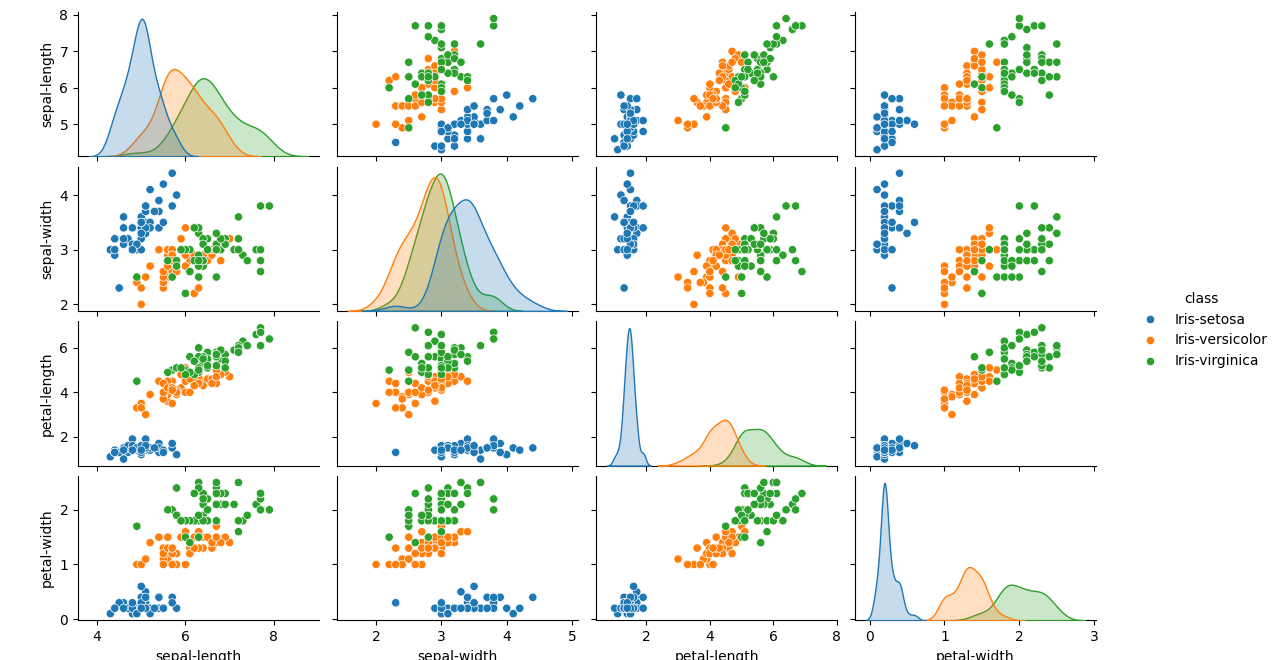
\includegraphics[width=0.9\textwidth]{picture/data}
	\caption{Data with feature}
	\label{fig:example}
\end{figure}
\subsection{Model Performance and Analysis}

\subsubsection{K-nearest neighbors}
\begin{enumerate}
	\item \textbf{Classifier Analysis}: The final KNN classifier achieved an impressive accuracy of 97\% on the test dataset, comprising 30 samples. This high accuracy indicates the model's effectiveness in classifying iris species based on their features.
\begin{figure}[h]
	\begin{minipage}{0.32\textwidth}
	\centering
	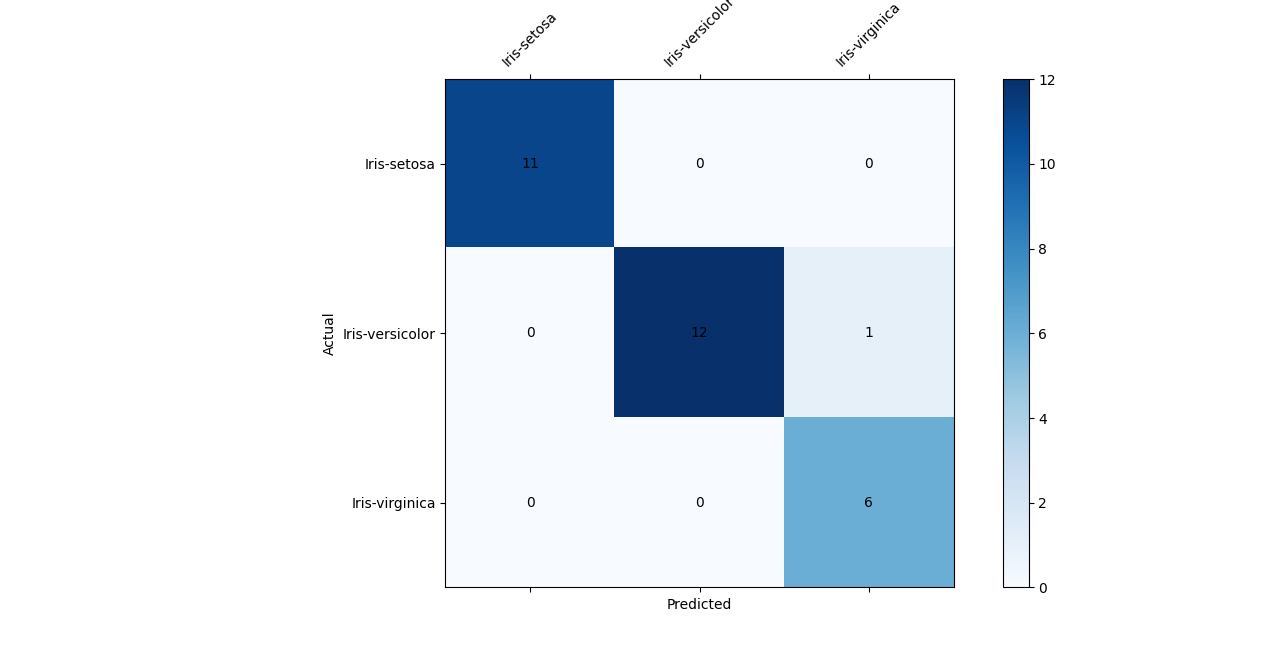
\includegraphics[height=4.2cm]{picture/KNN_confusion_matrix} % Adjust height as needed
	\caption{Confusion matrix}
	\label{fig:setosa}
\end{minipage}\hspace{3cm}
\begin{minipage}{0.32\textwidth}
	\centering
	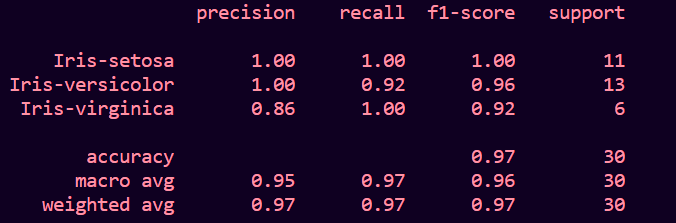
\includegraphics[height=3cm]{picture/KNN_Classifier_result} % Adjust height as needed
	\caption{Output result}
	\label{fig:versicolour}
\end{minipage}\hfill
\end{figure}

The confusion matrix further details the model's performance, revealing that only one instance of the Versicolor species was incorrectly classified. This insight is crucial for understanding the model's strengths and limitations in distinguishing between species.

\item \textbf{Regression Analysis}: For a regression perspective, the 'petal-length' feature was used to predict the species, converting species names to numerical values.
	\begin{figure}[h]
		\centering
		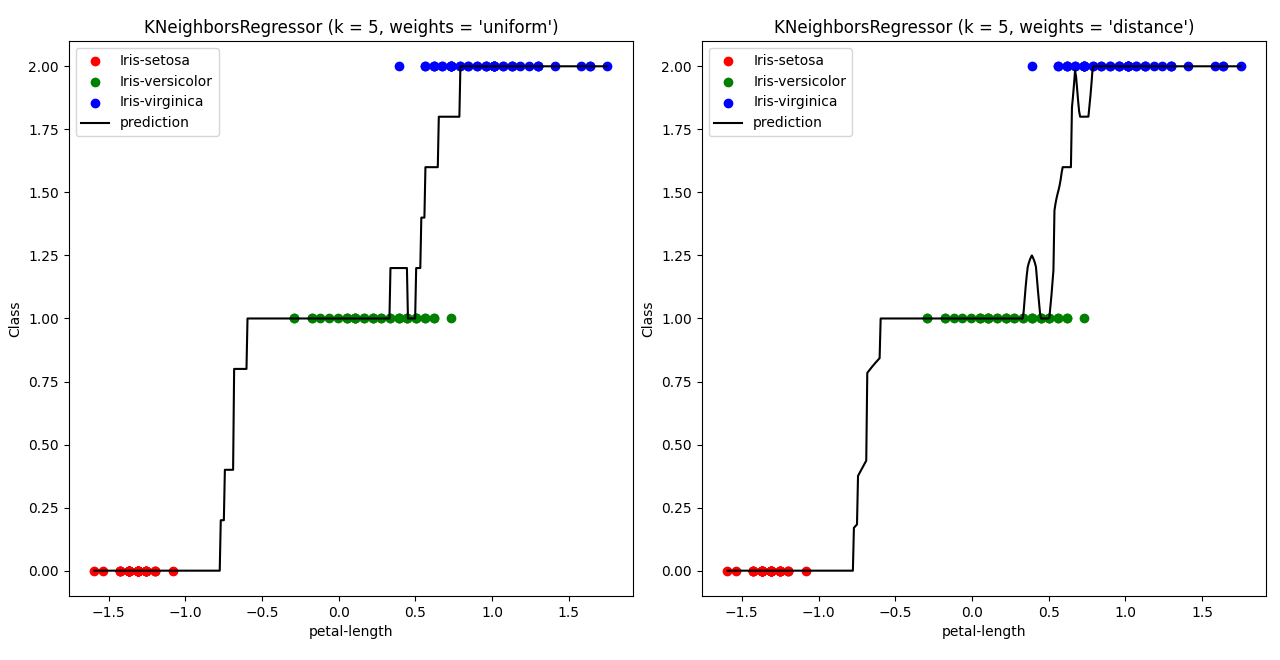
\includegraphics[width=1\textwidth]{picture/KNN_Regression_petal}
		\caption{Final result}
		\label{fig:example}
	\end{figure}
\end{enumerate}
 The results showed distinct clusters for each species after standard scaling of the data. Petal lengths below -1 were classified as Iris Setosa, lengths between -0.5 and 1 as Versicolor, and lengths above 0.5 as Iris Virginica. This demonstrates the relationship between petal length and species, highlighting the model's ability to discern patterns within the data.
\newpage
\section{Conclusion}
Summarize the main findings, the implications of your work, and any future work.

\section{References}
\href{https://machinelearningcoban.com/2017/01/08/knn/}{https://machinelearningcoban.com/2017/01/08/knn/}\\
\href{https://www.javatpoint.com/k-nearest-neighbor-algorithm-for-machine-learning}{https://www.javatpoint.com/k-nearest-neighbor-algorithm-for-machine-learning}
\end{document}

